\documentclass{beamer}

\usepackage[T1]{fontenc}
\usepackage{lmodern}
\usepackage{graphicx}
\usepackage{amsmath}
\usepackage{amssymb}
\usepackage{booktabs}
\usepackage{xcolor}
\usepackage{tikz}
\usepackage{array}
\usepackage{colortbl}
\usepackage[authoryear,round]{natbib}
\usepackage{ragged2e}

\usetheme{Madrid}
\usecolortheme{default}
\setbeamertemplate{navigation symbols}{}
\setbeamertemplate{footline}[frame number]
\setbeamersize{text margin left=0.6cm, text margin right=0.6cm}

\definecolor{myprimary}{HTML}{FF9D00}
\definecolor{mysecondary}{HTML}{FF8360}
\definecolor{mydark}{HTML}{243447}
\definecolor{mylight}{HTML}{FFF4E8}
\definecolor{mysoft}{HTML}{F7F7F7}

\setbeamercolor{structure}{fg=myprimary}
\setbeamercolor{title}{fg=white,bg=myprimary}
\setbeamercolor{subtitle}{fg=myprimary}
\setbeamercolor{frametitle}{fg=white,bg=myprimary!90}
\setbeamercolor{block title}{fg=white,bg=myprimary!85}
\setbeamercolor{block body}{fg=black,bg=mylight}
\setbeamercolor{normal text}{fg=mydark,bg=white}
\setbeamercolor{alerted text}{fg=mysecondary}

\setbeamerfont{title}{series=\bfseries,size=\Large}
\setbeamerfont{frametitle}{series=\bfseries,size=\large}
\setbeamerfont{block title}{series=\bfseries}
\setbeamertemplate{bibliography item}[text]
\setlength{\bibsep}{1pt plus 0.2ex}
\bibliographystyle{abbrvnat}

\newcommand{\lerobot}{\texttt{lerobot}}
\newcommand{\lerobotdataset}{\texttt{LeRobotDataset}}
\newcommand{\pizero}{\(\pi_0\)}
\newcommand{\highlight}[1]{\textcolor{myprimary}{\textbf{#1}}}
\newcommand{\statbox}[2]{%
  \begingroup
  \setlength{\fboxsep}{8pt}%
  \colorbox{mylight}{\parbox{\dimexpr\linewidth-2\fboxsep\relax}{\raggedright\textbf{\large #1}\\[-1pt]\small #2}}%
  \endgroup
}

\newcommand{\circled}[1]{%
  \tikz[baseline=(char.base)]\node[draw,circle,inner sep=1pt,thick](char){\textbf{#1}};%
}

\newcommand{\lightbox}[1]{%
  \tikz[baseline=(txt.base)]{
    \node[
      fill=myprimary!15,
      rounded corners=2pt,
      inner xsep=4pt,
      inner ysep=1.5pt
    ] (txt) {\strut #1};
  }%
}

\newcommand{\commonauthors}{%
  Francesco Capuano \and
  Caroline Pascal \and
  Adil Zouitine \and
  Thomas Wolf \and
  Michel Aractingi
}

\newcommand{\shortauthors}{%
  Francesco Capuano, Caroline Pascal, Adil Zouitine, Thomas Wolf, Michel Aractingi
}

\newcommand{\chaptertitleframe}[1]{%
  \begin{frame}[plain]
    \vspace{0.35cm}
    \begin{center}
      \begin{beamercolorbox}[wd=0.86\paperwidth,rounded=true,sep=10pt,center]{title}
        \usebeamerfont{title}\inserttitle
      \end{beamercolorbox}

      \vspace{0.55cm}
      {\Large\bfseries\textcolor{myprimary}{\insertsubtitle}\par}
      \vspace{0.15cm}
      {\small\color{mydark}\shortauthors\par}

      \vspace{0.45cm}
      
\includegraphics[height=1.0cm]{hf.pdf}
      \hspace{0.45cm}
      
\includegraphics[height=0.95cm]{oxford_logo.png}

      \vspace{0.55cm}
      \begin{beamercolorbox}[wd=0.8\paperwidth,rounded=true,sep=8pt,center]{block body}
        \small #1
      \end{beamercolorbox}
    \end{center}
  \end{frame}
}

\newcommand{\sources}[1]{%
  \vfill
  {\raggedright\tiny\color{black!65}\textbf{Refs:} #1\par}
}

\graphicspath{{../../../figures/}{../../../logos/}}

\title[Robot Learning Tutorial]{Robot Learning: A Tutorial}
\subtitle{Chapter 5: Generalist Robot Policies}
\author[Capuano et al.]{\commonauthors}
\date{}
\titlegraphic{
  \vspace{-1.1cm}
  
\includegraphics[height=1.4cm]{hf.pdf}
  \hspace{0.3cm}
  
\includegraphics[height=1.2cm]{oxford_logo.png}
}

\begin{document}

\chaptertitleframe{Why large multimodal backbones, open robotics datasets, and efficient action experts are enabling generalist robot policies.}

\begin{frame}{Roadmap}
  \begin{enumerate}
    \item Why robotics is shifting from specialist to generalist policies
    \item What modern vision-language-action models look like
    \item \pizero{} as a large-scale VLA
    \item SmolVLA as a compact open alternative
  \end{enumerate}
\end{frame}

\begin{frame}{From Specialist Policies to Foundation Robotics}
  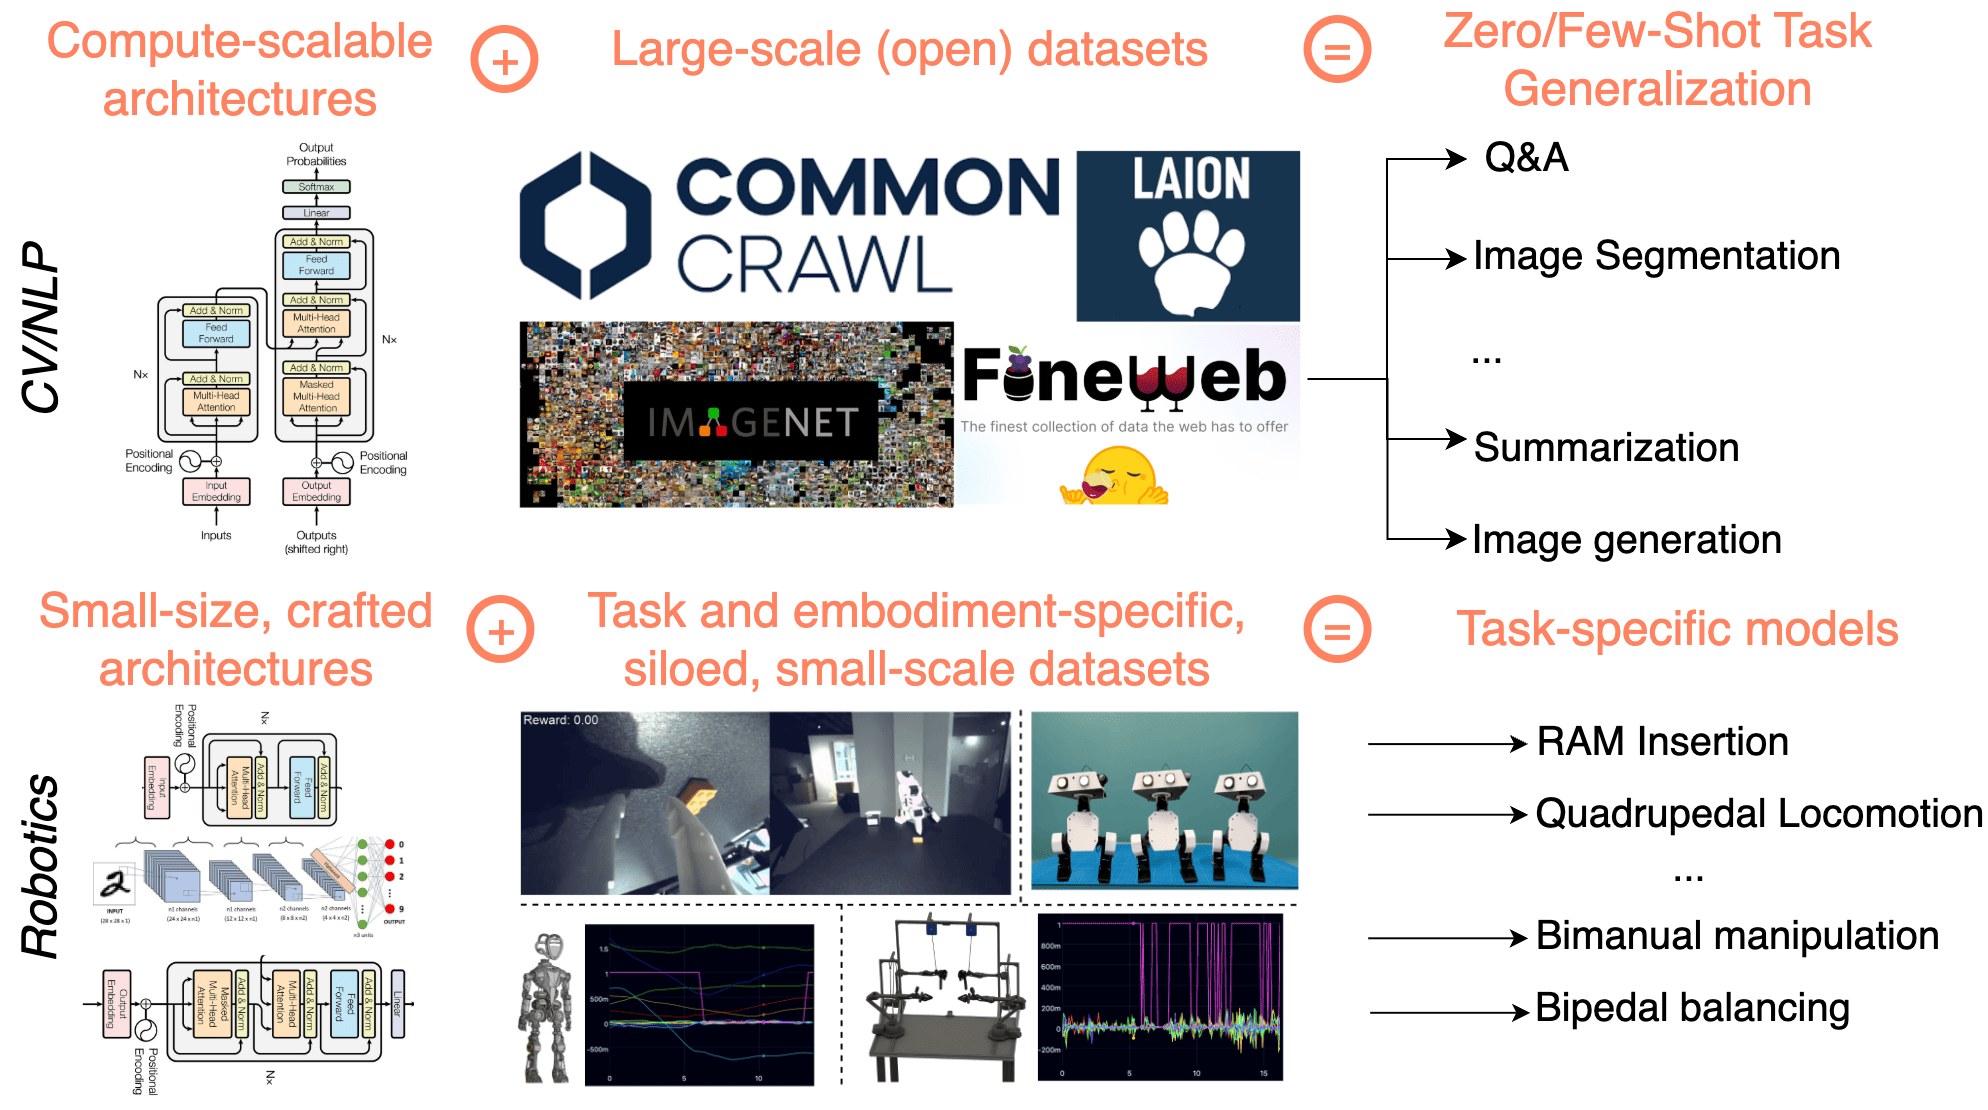
\includegraphics[width=\linewidth,height=0.65\textheight,keepaspectratio]{ch5/ch5-ml-vs-robotics-foundation.png}
  \begin{itemize}
    \item CV and NLP converged on pretrain-and-adapt regimes much earlier than robotics.
  \end{itemize}
\end{frame}

\begin{frame}{Why Robotics Lagged}
  \begin{itemize}
    \item Robotics data is \highlight{embodied}: tied to a task, a robot, and a deployment setting.
    \item Demonstrations are expensive, heterogeneous, and harder to aggregate than text or images.
    \item That fragmentation historically favored specialist models over generalist ones.
  \end{itemize}

  \vspace{0.25cm}
  \statbox{Key shift}{Large aggregated datasets and more stable architectures are finally making generalist robot policies plausible.}
\end{frame}

\begin{frame}{The Timeline of Generalist Policies}
  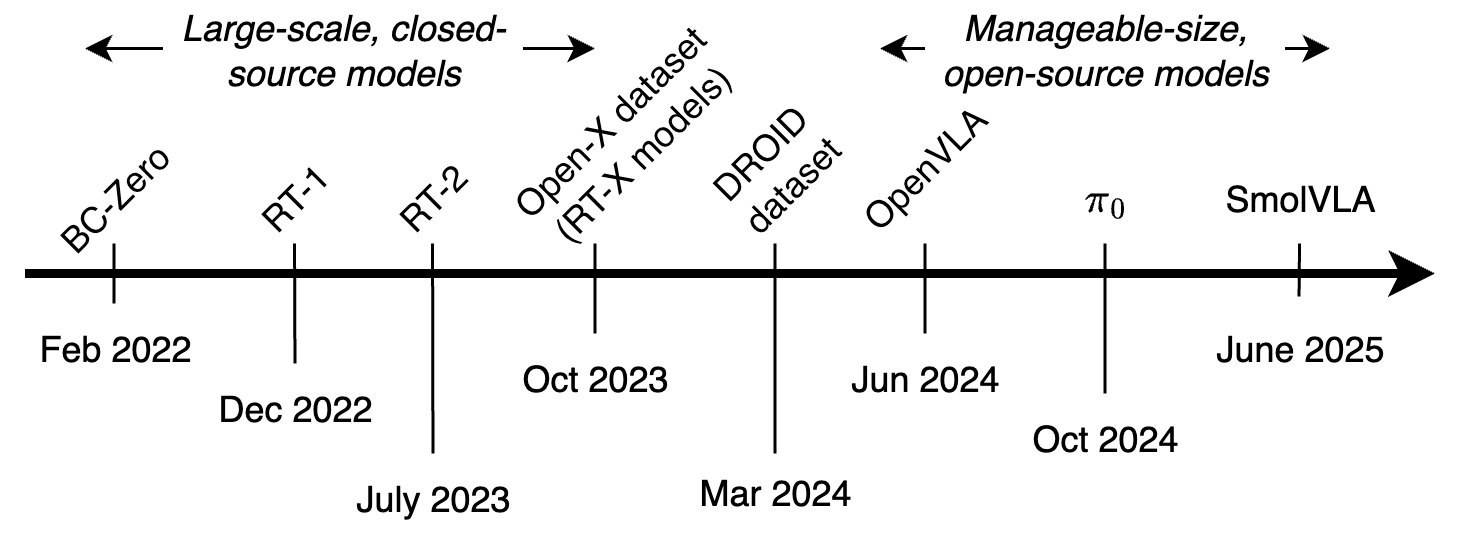
\includegraphics[width=\linewidth,height=0.65\textheight,keepaspectratio]{ch5/ch5-generalist-policies-timeline.png}
  \begin{itemize}
    \item The field has moved from tens of thousands of demos toward multi-million-trajectory regimes.
  \end{itemize}
  \sources{\citep{jangBCZZeroShotTask2022,brohanRT1RoboticsTransformer2023,brohanRT2VisionLanguageActionModels2023,kimOpenVLAOpenSourceVisionLanguageAction2024,black$p_0$VisionLanguageActionFlow2024,shukorSmolVLAVisionLanguageActionModel2025}}
\end{frame}

\begin{frame}{Open Data Changes the Equation}
  \begin{columns}[T,onlytextwidth]
    \begin{column}{0.52\textwidth}
      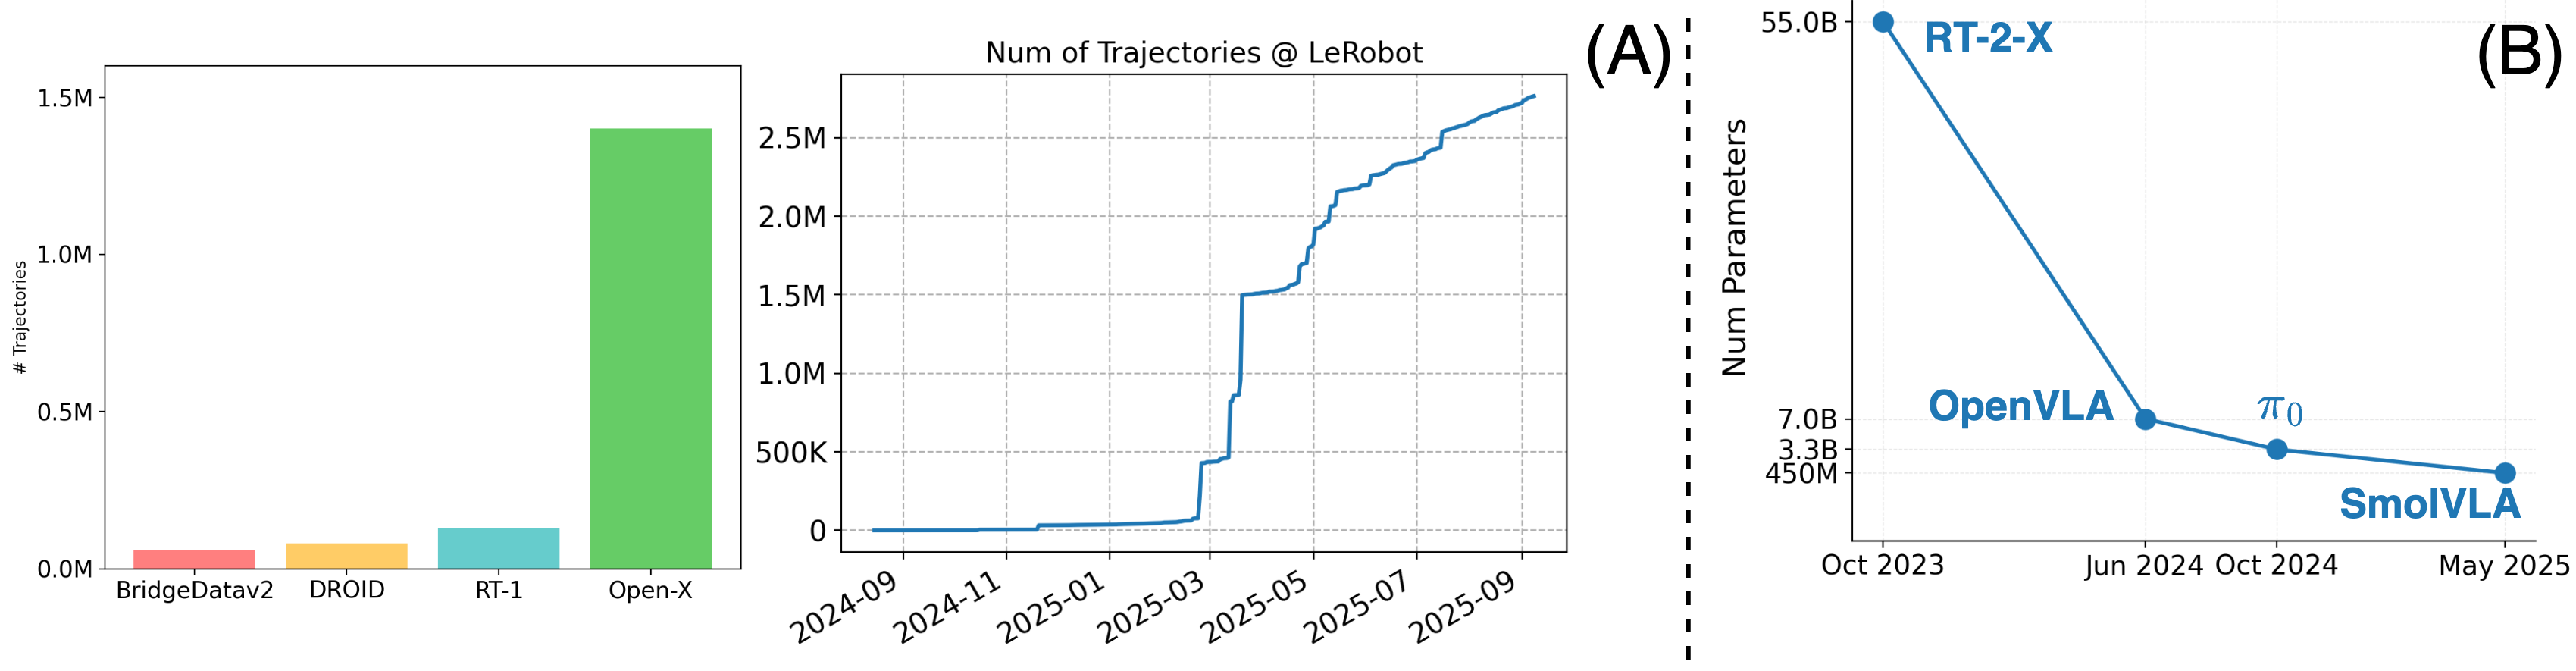
\includegraphics[width=\linewidth]{ch5/ch5-trends.png}
    \end{column}
    \begin{column}{0.44\textwidth}
      \begin{itemize}
        \item Open X-Embodiment and DROID reduced the data bottleneck.
        \item Community-contributed datasets make decentralized collection viable.
        \item Models are also becoming smaller and easier to deploy.
      \end{itemize}
    \end{column}
  \end{columns}
  \sources{\citep{oneillOpenXEmbodimentRobotic2025,khazatskyDROIDLargeScaleInTheWild2025}}
\end{frame}

\begin{frame}{What Makes a Modern VLA}
  \begin{itemize}
    \item A pretrained \highlight{vision-language backbone} for semantics and perception
    \item A dedicated \highlight{action expert} for continuous control
    \item Action chunking to reduce compounding errors
    \item Generative objectives such as flow matching for multimodal continuous actions
  \end{itemize}

  \vspace{0.2cm}
  \statbox{Why this is different}{Modern VLAs avoid discrete action-token bottlenecks and inherit world knowledge from large multimodal backbones.}
\end{frame}

\begin{frame}{Why VLMs Matter for Robotics}
  \begin{itemize}
    \item VLMs bring visual semantics, language grounding, and world knowledge learned from internet-scale corpora.
    \item That reduces the need to learn all perception and language concepts from scratch inside robotics datasets alone.
    \item It also opens the door to instruction-conditioned generalization across tasks.
  \end{itemize}
\end{frame}

\begin{frame}{\pizero: A Large-Scale VLA}
  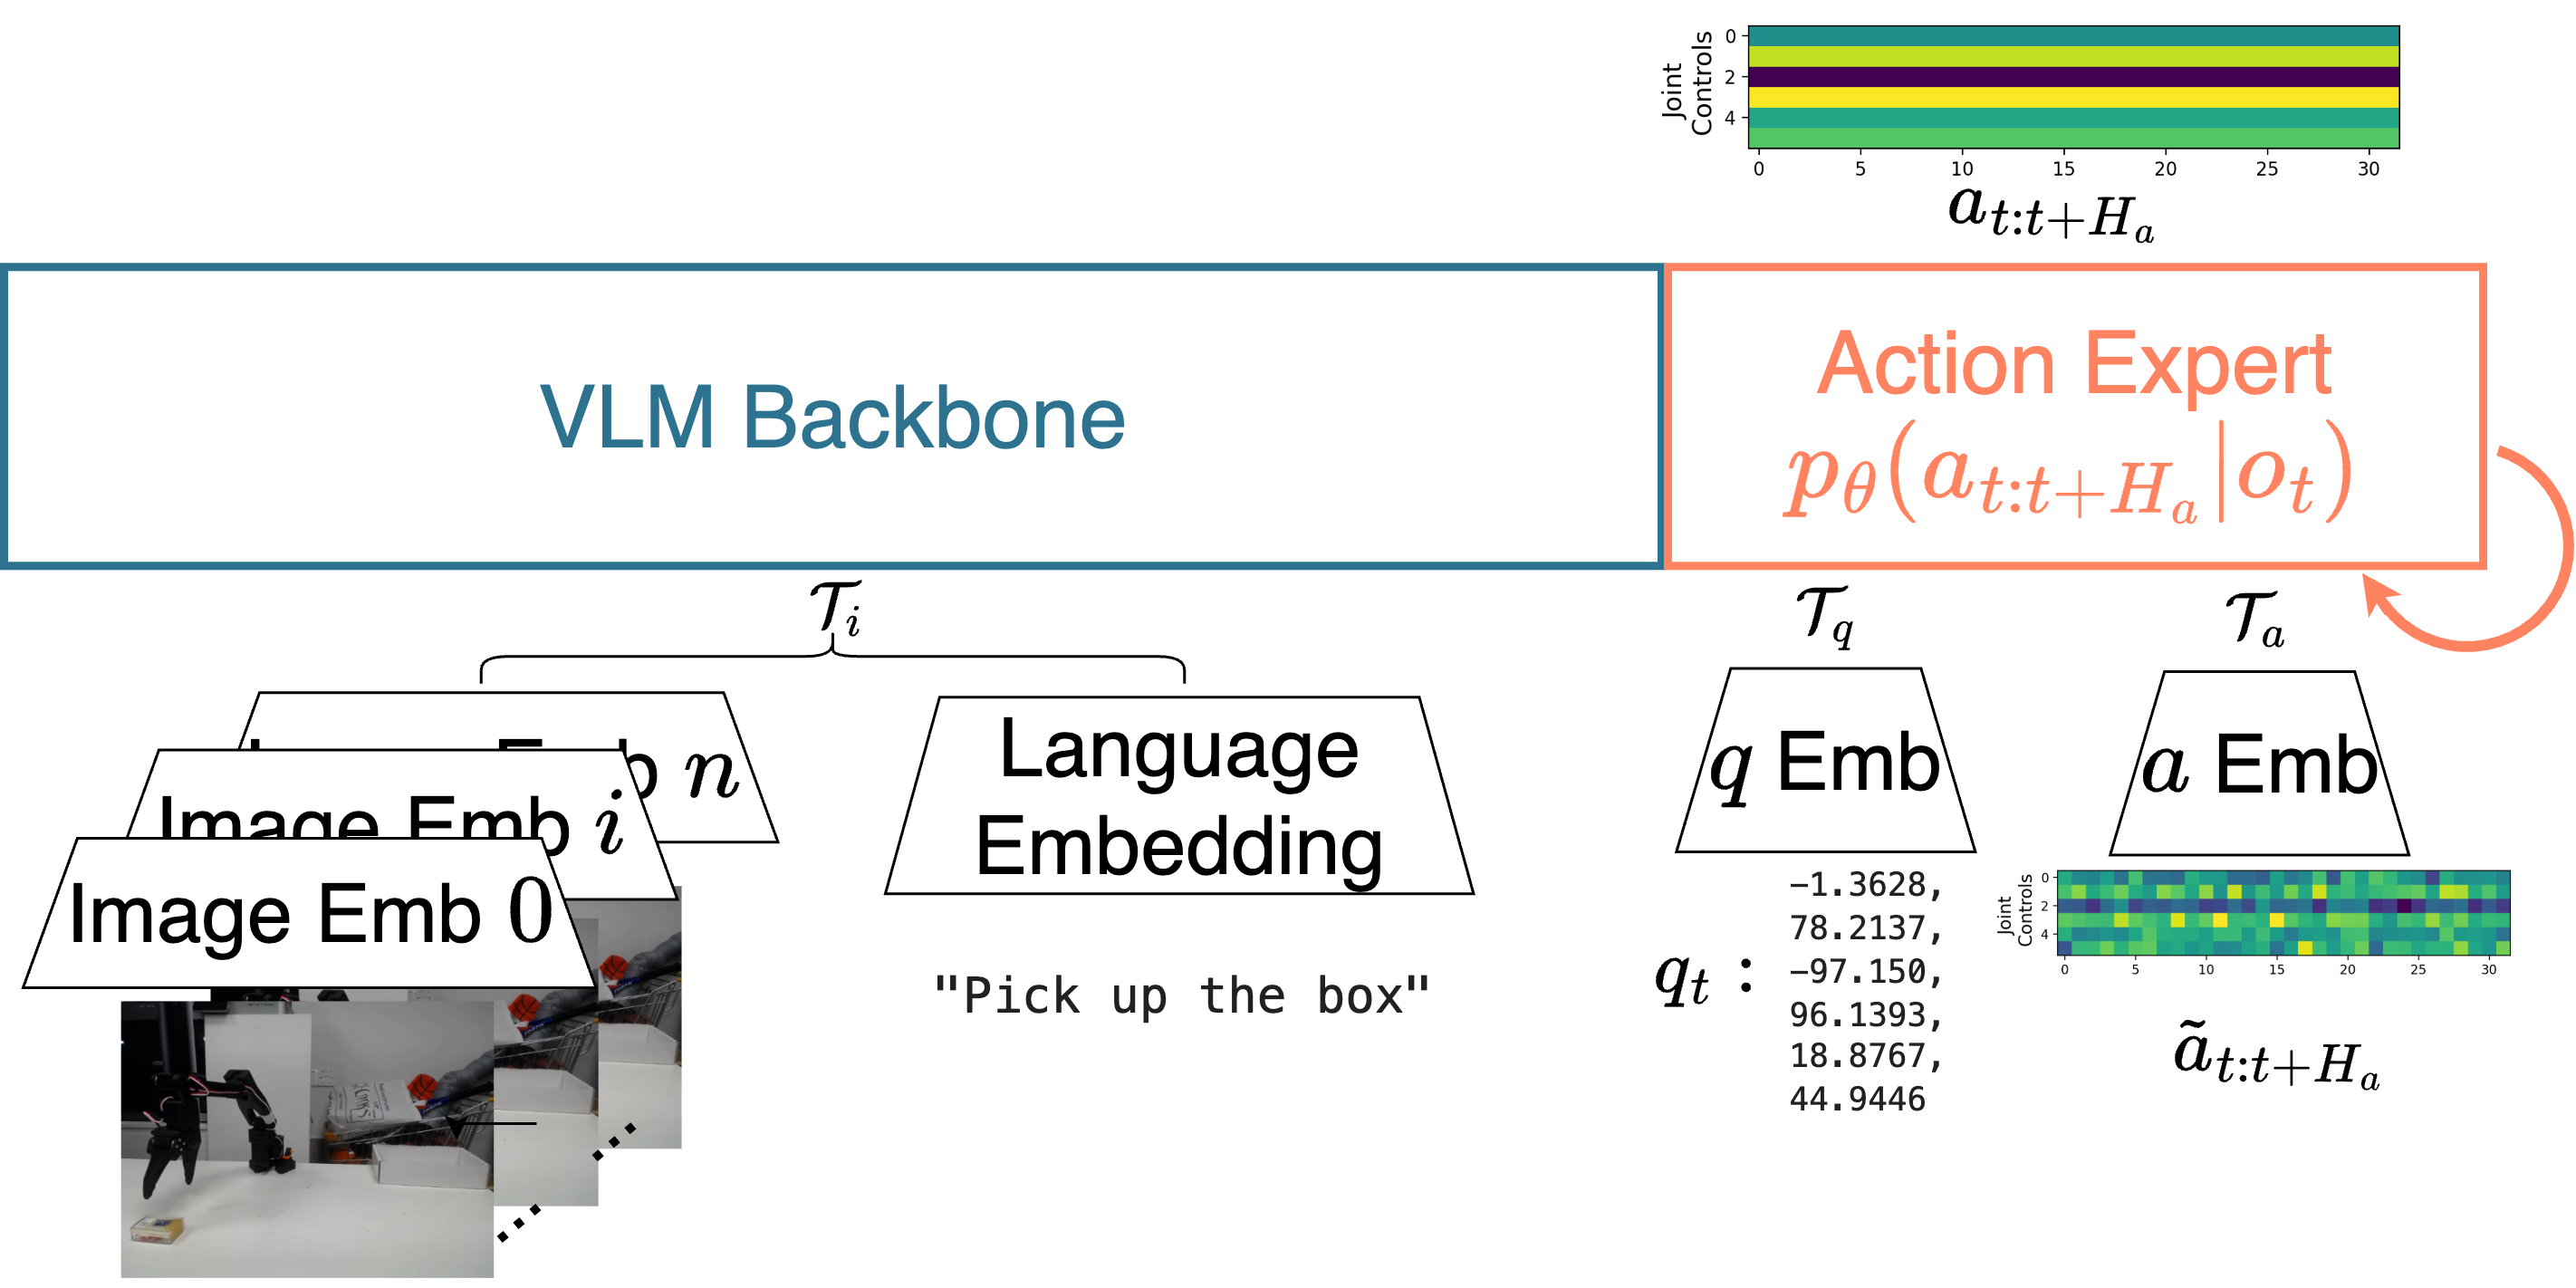
\includegraphics[width=\linewidth,height=0.6\textheight,keepaspectratio]{ch5/ch5-pi0.png}
  \begin{itemize}
    \item \pizero{} combines a Gemma-based VLM backbone with a smaller action expert.
    \item Tokens are partitioned into image-language, proprioception, and action blocks.
  \end{itemize}
  \sources{\citep{black$p_0$VisionLanguageActionFlow2024}}
\end{frame}

\begin{frame}{What \pizero{} Optimizes For}
  \begin{columns}[T,onlytextwidth]
    \begin{column}{0.36\textwidth}
      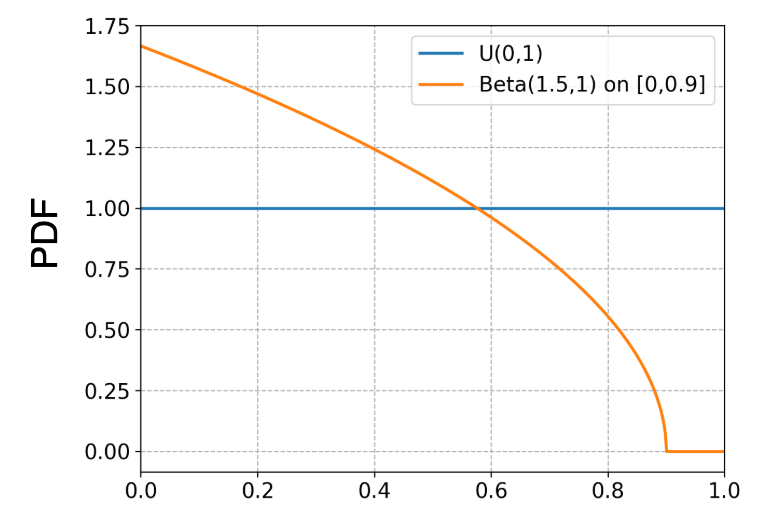
\includegraphics[width=\linewidth]{ch5/ch5-pi0-sampling-timesteps.png}
    \end{column}
    \begin{column}{0.6\textwidth}
      \begin{itemize}
        \item Flow matching over continuous action chunks
        \item Blockwise masking to preserve VLM specialization and enable KV caching
        \item Ten-ish denoising steps at inference rather than long diffusion chains
        \item Pretraining on a very large mixed dataset, then fine-tuning on narrower high-quality data
      \end{itemize}
    \end{column}
  \end{columns}
\end{frame}

\begin{frame}{Why \pizero{} Matters}
  \begin{itemize}
    \item It demonstrates few-shot and cross-embodiment behavior from a single architecture.
    \item It also shows the value of pretraining on \highlight{large, diverse robotics mixtures} before task-specific adaptation.
    \item But it remains compute-heavy and only partially open because most of its training data is not public.
  \end{itemize}
\end{frame}

\begin{frame}{SmolVLA: Compact and Open}
  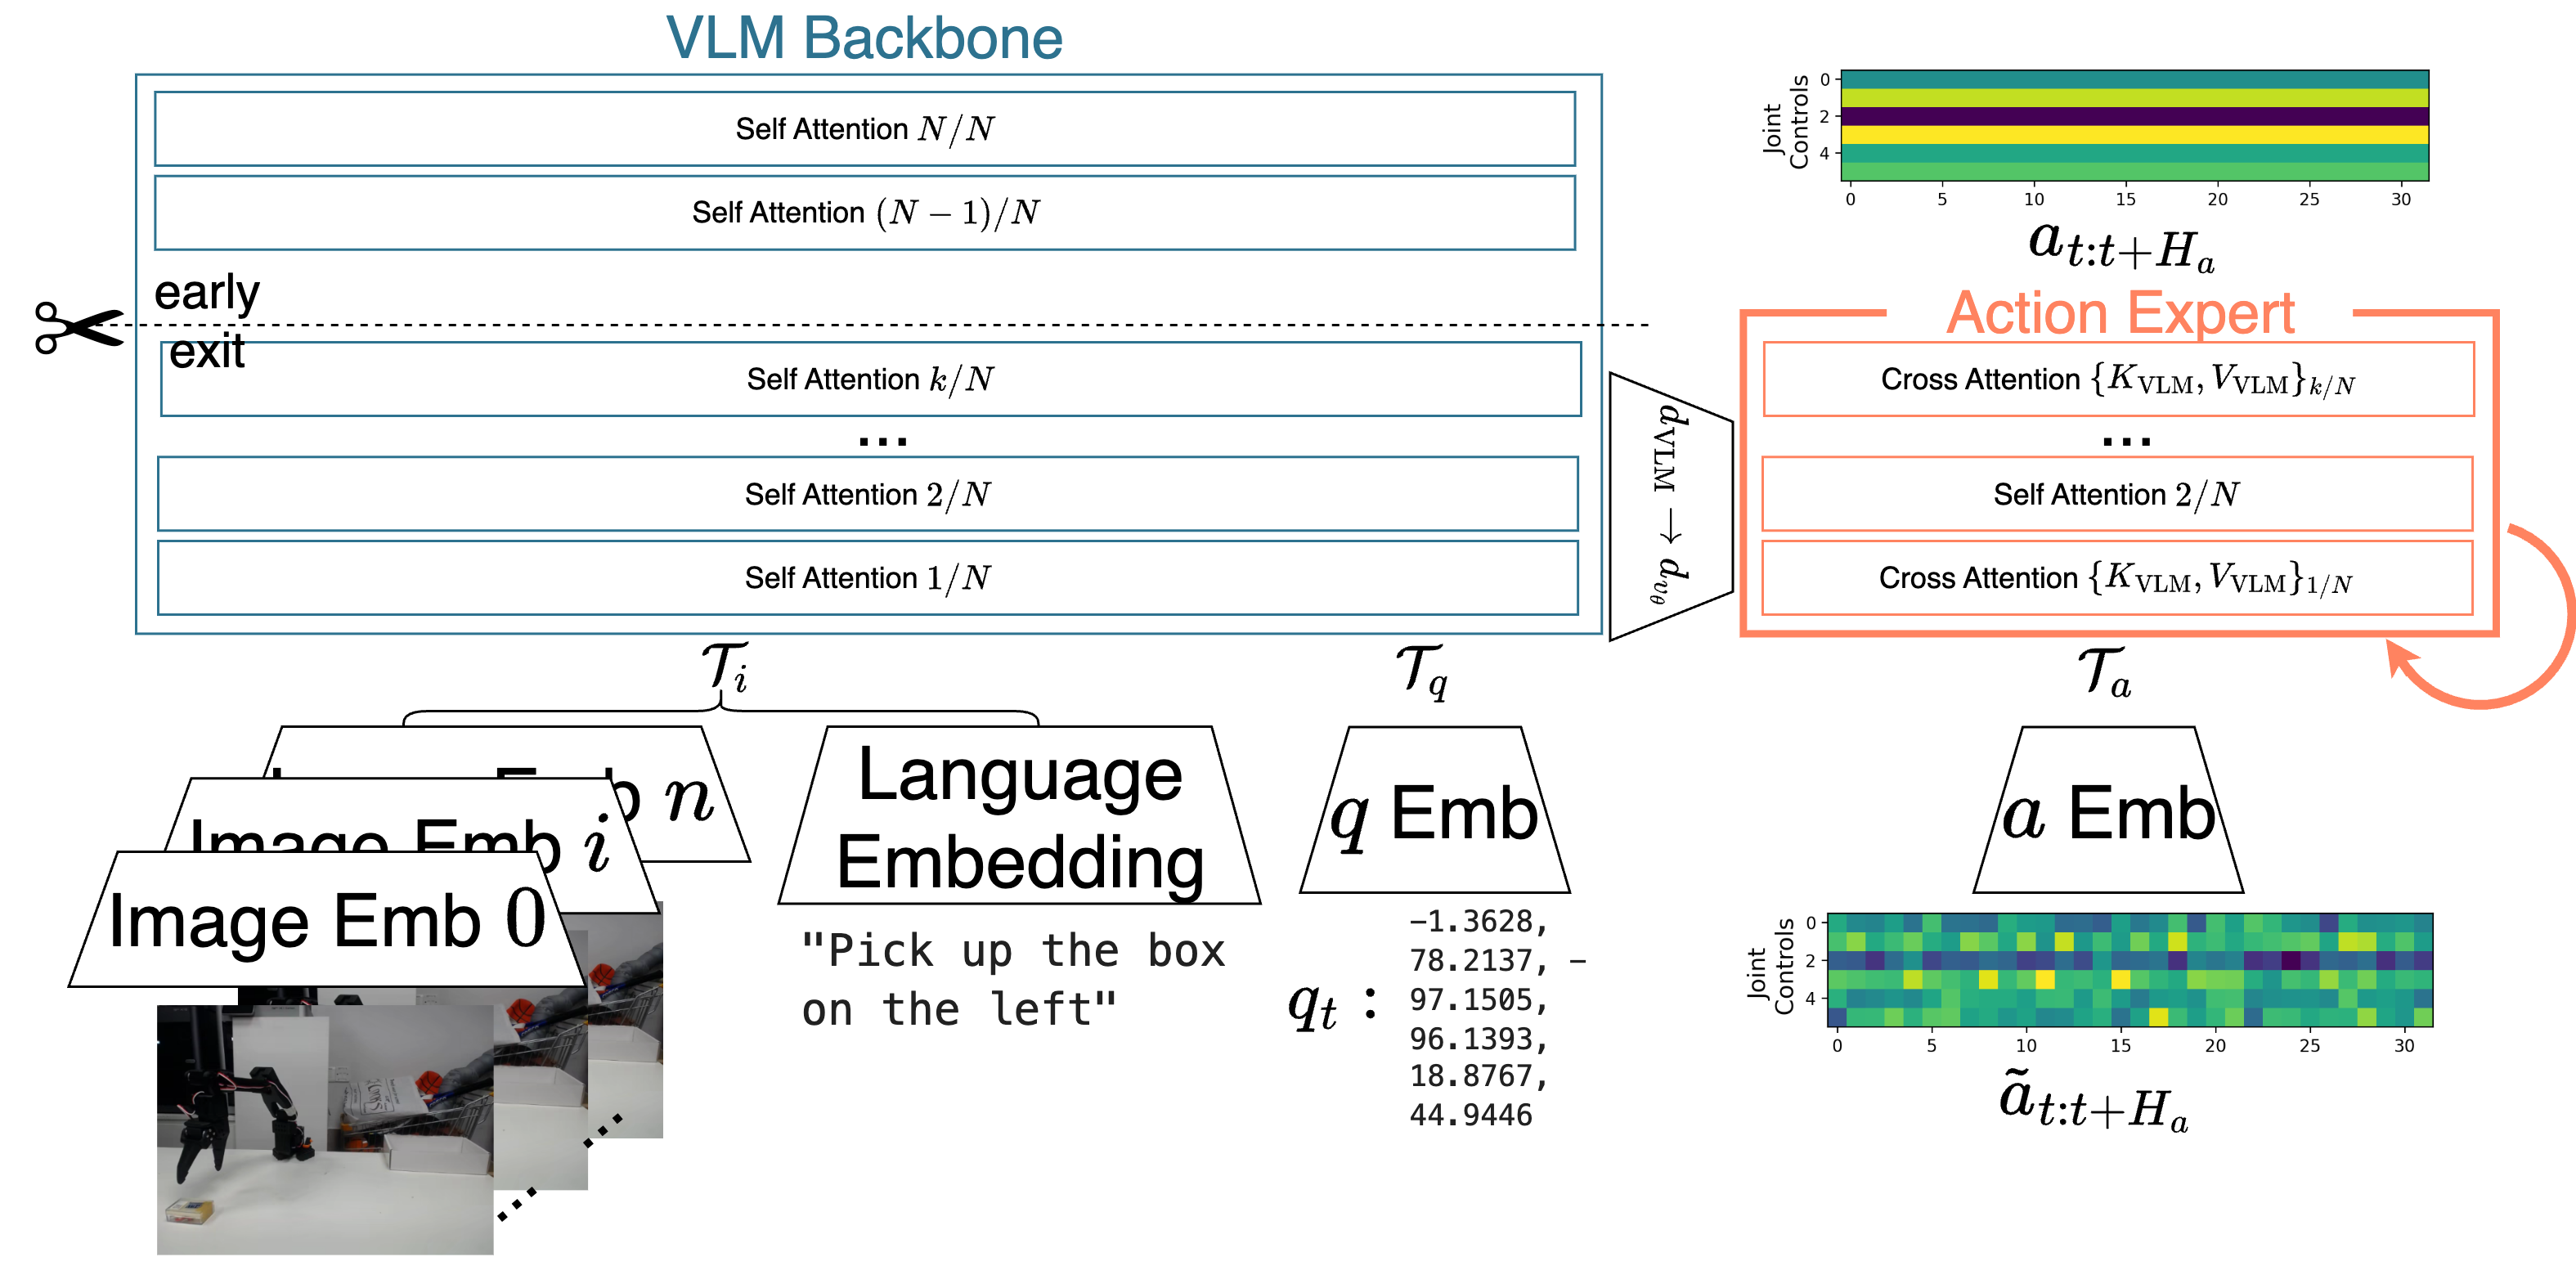
\includegraphics[width=\linewidth,height=0.6\textheight,keepaspectratio]{ch5/ch5-smolvla.png}
  \begin{itemize}
    \item SmolVLA keeps the MoE pattern but pushes hard on \highlight{efficiency and openness}.
  \end{itemize}
  \sources{\citep{shukorSmolVLAVisionLanguageActionModel2025}}
\end{frame}

\begin{frame}{How SmolVLA Stays Practical}
  \begin{itemize}
    \item Smaller VLM backbone and smaller action expert
    \item Reduced visual token budget and skipped upper VLM layers
    \item Cross-attention/self-attention interleaving for efficient conditioning
    \item Pretraining on 450+ community datasets rather than proprietary mixtures
  \end{itemize}

  \vspace{0.2cm}
  \statbox{Result}{SmolVLA targets the same frontier as larger VLAs while staying much cheaper in memory and deployment cost.}
\end{frame}

\begin{frame}{Using Generalist Policies in \lerobot}
  \begin{block}{Reference snippets}
    \texttt{snippets/ch5/01\_using\_pi0.py} and \texttt{snippets/ch5/02\_using\_smolvla.py}
  \end{block}

  \begin{itemize}
    \item The tutorial's practical message is that foundation-style policies are no longer purely conceptual.
    \item They can already be consumed through the same open tooling ecosystem as smaller BC and RL methods.
  \end{itemize}
\end{frame}

\begin{frame}{Closing: What Openness Enables}
  \begin{itemize}
    \item The field is moving from handcrafted, siloed systems toward shared datasets, reusable architectures, and open software.
    \item Progress now depends on \highlight{open data, open tooling, and reproducible training recipes} as much as on model novelty.
    \item That convergence is what makes robot learning feel increasingly like the early stages of foundation-model development in other ML domains.
  \end{itemize}

  \vspace{0.25cm}
  \statbox{Final takeaway}{From classical control to RL, BC, and VLAs, the through-line of the tutorial is that openness and scale are becoming the central accelerants for modern robot learning.}
\end{frame}

\begin{frame}[allowframebreaks]{Selected References}
\scriptsize
\bibliography{../shared/references}
\end{frame}

\end{document}
